\chapter{Reflection \& Conclusion}
\section{Planning and Management of Work}
By using GitHub Issues and Pull Requests, planning and management of work was a relative success. Work on the project was done consistently during the allocated time frame, and when no changes were made to the repository, that meant research was still being done. 

\section{Project Achievements}
I believe I've successfully achieved everything I aimed for in the beginning of the project. All the features, both functional and non-functional were met. Additionally, my objectives outlined in the first chapter were generally achieved. I gained a deeper understanding of CAs in general, in addition to honing my relatively forgotten skills in HTML JS. More importantly, the system was built and it scales relatively well in a linear fashion, albeit its slow times. 
\\ \\
Through the interviews conducted, I believe I've received mostly positive feedback from the interviewees regarding my project, although the approach could have been much better. I feel a sense of achievement when the participants naturally understood the rules and how I defined them, despite the little moments of confusion that was displayed initially and oftentimes when new concepts were introduced. I am grateful to have received constructive feedback from both my supervisor, my interview participants, and everyone else I consulted along the way. 

\section{What Went Wrong} \label{whatwentwrong}
This section delves on to the changes towards the development process. Changes that I would make if I were to repeat the project would be:
\begin{itemize}
    \item \textbf{Integration of Trello Boards and More Extensive Notetaking}: Planning and Management of work could have been greatly improved by Trello Boards or GitHub projects to better visualize which stage each component was at. This would have been a more streamlined approach when compared to purely using GitHub Issues, not to mention this process was a lot faster than individually creating issues. A great deal of notes were also scattered, I lacked a dedicated notebook for project note taking, and information I received through online resources only sat in my head. By having a dedicated project notebook, the planning process could have probably been done in half the time required. 
    \item \textbf{Change in Approach for Rule Format Development}: Though the management of work was relatively flawless as were the achievements, one thing I would definitely change during the development stage was the approach taken in doing the project. My approach in developing the rules format was bottom-up. Upon starting the project, I studied extensively the rules of CGOL, and implemented features based on that functionality. As a result, the rules format were somewhat rigid. The state transition rules only gave two choices of states to transition into. If I could start over entirely, I would have taken more time to research CAs and think of a way to provide more state transition choices.
    \item \textbf{Consistently ask for Feedback from the Audience}: Also dealing with the rules at another angle, if I were to gather constant feedback throughout the development, then the rule format would have probably been different, when coupled with Another most The entire development process was somewhat closed-loop. The End-users (target audience of Computer Science University Students) were not at all involved in the development stage. The lack of consistent feedback from my intended end-users then resulted in a rules format that is relatively lacklustre. 
    \item \textbf{Give more thought on Testing - Create a Test Suite}: There was also a lack of standardized testing procedure during the development of the project. The current workflow only switches between GitHub version commit hashes to identify any breaking changes if present in the main development branch. There was no unit testing, integration testing, or regression testing. Therefore, another aspect that I would change if I were to start over would be to spend some time in the beginning to design and develop a testing suite for the project. Time invested in developing a test suite will surely save the amount of time needed in creating and integrating new features. 
\end{itemize}
Additionally, under mitigating circumstances, this project's deadline was extended until the end of the second semester exam period. 

\section{Potential Extension Work} \label{potential_extension_work}
This section outlines potential features that could be implemented in the final product, but unfortunately didn't make the final submission release. Assuming the project was started/restarted correctly with the lessons learnt in the previous section (\ref{whatwentwrong}) up until this point in the final code, the following extra features are what I would like to implement in my project. 

\subsection{Improved Rules Documentation Page}
The documentation (rules help page) was truthfully created as an afterthought. There are discrepancies in the syntax, and oftentimes they are not descriptive enough. Although both participants in the chapter previous has outlined the usefulness of the rules format, much can be done to improve the comprehension and quality of information delivered by the help page. Especially after potentially improving the rules format to add more support. 

\newpage
\subsection{Adding a Description Field for CA Rules States}
As outlined in Section \ref{analysis_suggestions}, adding a description field to indicate what type of state is related to the number would greatly reduce confusion and complexity. The additional field, call it \texttt{state\_name}, can be placed at the same level as the \texttt{next} key in every state object. In the example of CGOL rules at state 0 (Dead state):
\begin{center}
\begin{figure}[H]
\begin{verbatim}

                            "0": {
                                "state_name": "dead",
                                "next": {
                                    "conditional_requirements": [
                                        {
                                            "type": "totalling",
                                            "neighbour_state": 1,
                                            "total": [
                                                3
                                            ]
                                        }
                                    ],
                                    "satisfied": 1,
                                    "else": 0
                                }
                            },
    
\end{verbatim}
\caption{CGOL State Transition Rule when state is 0 (dead), with description field}
\end{figure}
\end{center}
\noindent Notice the new key right before \texttt{next}.
\\ \\
Additionally, some changes to the JSON Schema will need to be made as well. In Appendix \ref{appendix:jsonschema}, the following line will need to be updated in the \texttt{\$defs/state/properties}: 
\begin{center}
\begin{figure}[H]
\begin{verbatim}

                            state_name: { 
                                type: "string"
                            }
    
\end{verbatim}
\caption{Line to be added to \texttt{state} property in the JSON Schema}
\end{figure}
\end{center}
\subsection{Integrating Number of States Count to the Rules Only}
This issue was also mentioned in Section \ref{analysis_suggestions}. The current implementation requests the user to separately input the number of states in both the JSON rules, and the text field above it. The reason behind this implementation is that the \texttt{\$\_meta} field containing state number and colors were an afterthought. This discrepancy was shed to light after the code freeze.  
\\ \\
Changes to the implementation would be to simply erase the textarea input field, and assign the value from \texttt{num\_states} to the variable that was supposed to contain the value obtained from the previously removed input field.

\subsection{Validator Enhancement: Check Parse Errors/Failures}
In most use cases, the validator provides the feedback to the user-specified rules. However, there have been cases during arbitrary utilization involving the rules that the simulator simply stopped working due to an error in the validator. The current implementation simply parses values from the text editor to the as a JSON object value from the textarea to the validator, with a general assumption the syntax is correct. However, that is oftentimes rarely the case.
\\ \\
In the text area, the opening and closing curly braces (first and final lines) can be removed to provide the users a more aesthetic feel and prevent accidental deletion from them. These two characters can then be pre-pended and post-pended before being parsed as a rule. Additionally, a simple try-catch statement can be integrated at the appropriate component (i.e. the Validator component, see \ref{validator}) to check its parse quality. 

\subsection{Reversible Cellular Automata}
The current implementation of the simulator only covers totalistic and probabilistic CAs. Reversible CAs, on the other hand, state that for every configuration of the grid, there is a unique predecessor to its configuration \cite{gutowitz1991cellular}. Reversible CAs are often used in physics, particularly in gas and fluid dynamics \cite{toffoli1987cellular}. A special rule of the CA called \textit{Critters} developed by Tofolli \cite{toffoli1987cellular} is reversible. Implementing this feature will enable more universality as it allows additional simulation styles. 

\subsection{Undo Command}
Taking inspiration from reversible CAs from the subsection previous, and "undo" button can be implemented to clarify if the user-defined rules behave as specified. This functionality allows testing the randomness of the implemented transition rules, or simply debugging a rule when the user wants to keep the initial state (or previous state) of the entire grid. 
\\ \\
In terms of implementation, a separate finite list (Array) containing the current CA's grid (as a 2D array) and also the grid from a few steps before can be used as a temporary memory space. \\ \\
Alternatively, a stack can be used in place of the Array for the same purpose. Undoing the applying of the transition rule to the grid (i.e. going back one generation) can mean a pop of the stack, and assigning that value to it. "Undo" commands commonly use the stack \cite{karimov2020stacks}. 

\subsection{Support for Defining CA Grid Dimensions}
The system currently generates a grid based off the user's screen size and resolution. This therefore doesn't allow for larger scale simulations. Two basic text fields accepting numbers can be used as user's input to specify its row and column numbers, then be utilized in the simulation and models. 
\\ \\
Cell sizes should also have the capability of being automatically scaled down, in order to fit more cells in the provided square. This functionality can be added to the \texttt{sketcher} bit of my written library, scaling down the square's (cell's) size by the grid dimensions and provided simulator frame size. 

\subsection{Support for User-Defined Initial States and Clickable Grid}
For some CAs that are used for prediction (e.g. population dynamics, ecological growth), initial states may be crucial to test the robustness of the defined CA rules, after a few generations. For example, the implementation of CAs for population dynamics outlined by Mavroudi \cite{mavroudi} rely on a certain city-style grid. 
\\ \\
Activating these presets can be done by the click of a button, similar to how the current implementation of \texttt{Firesim} works. The only difference would be instead of calling a function to randomly generate states of the cells, the button loads a predetermined two-dimensional array with the appropriate number of states. 

\subsection{Support for Variable Grid Density}
The \texttt{random} button in the program purely allocates states randomly. This means that each state in the \textit{state space} (see section \ref{state_space}) all have an equal chance of being considered in the randomization process. Minor changes to the actuator class can be made in order to provide support for grid density. 
\\ \\
By using the predefined probability calculator function in the Function Builder Component (see \ref{prob_calc_fbuilder}), instead of randomly allocating states to the cells, some states may have a larger probability of being assigned to a cell. Input can be taken by creating a new textarea where the value should be a floating point number between 0 and 1.

\subsection{Support for more Complex Probability Rules}
The current implementation of rules only allows for two types of probability, i.e. \texttt{probability} and \texttt{total-p}. The latter when implemented on the forest fire propagation simulation briefly touched upon the idea of a probability distribution. This means that the more of a cell's neighbours is on fire, the more likely the cell in test will burn. 
\\ \\
A method of specifying a custom probability function can be implemented by allowing the user to write probability functions in JavaScript, then pass that written function to the anonymous function builder. However, this might add an additional layer of complexity towards the users. Therefore an additional user-defined rules format specifically for writing probabilities may need to be developed again. 

\newpage
\subsection{Support for Different Neighbourhood Types}
In addition to the Moore-type neighbourhood defined in \ref{moore_neighbourhoods}, another commonly used neighbourhood type is the Von-Neumann Neighbourhood, shown below:
\\
\begin{figure}[h]
    \caption{Moore Neighbourhood (left) and Von-Neumann Neighbourhood (right) \cite{toffoli1987cellular}}
    \centering
    \label{moore_vs_vn}
    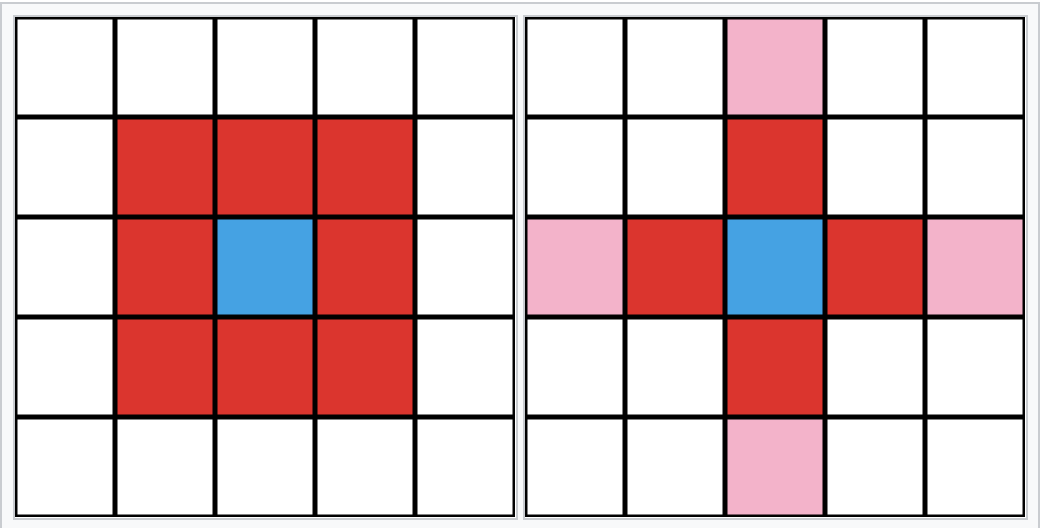
\includegraphics[scale=0.70]{neighbour_differences.png}
\end{figure}
\\
In contrast to the Moore Neigbourhood, the Von Neumann Neighbourhood only considers the adjacently placed cells of a cell in the center. Like the Moore Neighbourhood, the Von-Neumann neighbourhood may also consider the search depth of the neighbours, also defined as the manhattan distance from the center cell. On the right-hand side of the Figure \ref{moore_vs_vn} above, for the Von-Neumann neighbourhood, the red cells are Von-Neumann neighbours of manhattan distance \textit{r} = 1, whereas the pink ones are of \textit{r} = 2.
\\ \\
In terms of changes towards the implementation, the JSON Schema fed to the validator will need to add a required neighbour-type field in the \texttt{conditional\_requirements} property, particularly in the \texttt{reqs\_list} to validate the neighbourhood type. In the actuator component, another function (e.g. \texttt{count\_vn\_neighbours()}) can be written beside the default \texttt{countNeighbours()} (change to perhaps \texttt{count\_m\_neighbours()}). Once these functionalities are implemented, this will allow the function builder component to return a new anonymous function implementing the functionality of the Von-Neumann Neighbourhood. 
\\ \\
Once implemented, the Von-Neumann Neighbourhood may serve as a basic building block of defining the notion of 4-connected pixels in the field of computer graphics \cite{wilson2000handbook}, adding more levels of universality to the simulator.
\newpage

\section{Conclusion and Personal Achievements}
Considering the amount of time that was spent researching and developing for the project, I learned a great deal throughout the entire process. Revisiting HTML and JS was a rewarding experience for me as it has been quite a while since I've developed using those languages. I gained invaluable experience as well, particularly in conducting qualitative interviews to evaluate. Overall, this learning experience was extremely rewarding for me as I got to push my boundaries and nurture my resourcefulness. So many things that I didn't expect to learn by studying Computer Science. This experience and lessons learnt are invaluable, and I will certainly keep pushing my boundaries and abilities as I did from this project's start to finish.